\section{Natural Clouds}
Clouds are a substantial part of Earth's weather. They provide shade from the glistening sun on hot days and reflect the heat at night, keeping the ground warmer.
Even for a layman, clouds are comprehensible and useful indicators for telling the weather.
If they are dark and low-hanging, they usually bring rain.
If they are puffy and scarce, they predict fair weather ahead.

\subsection{Convection}
\label{section:clouds:convection}
In meteorology, \gls{convection} describes the event of atmospheric motions in the vertical direction.
Hot air rises from Earth's surface in form of bubbles, which are called \emph{\gls{thermal} columns} or just \emph{\gls{thermal}s}.
As the \gls{altitude} increases, the \gls{thermal}'s air cool down. At some point, the warm air diluted by the surrounding colder air, after which its moisture condenses and starts forming clouds \cite{weather:convection}.

\begin{figure}[H]
    \centering
    \begin{tikzpicture}[scale=1.2]
        \tikzset{edge/.style = {-{Latex[length=3mm]},shorten >= -4pt}}
        \tikzset{shortedge/.style = {-{Latex[length=3mm]},shorten <=-4pt,shorten >= -4pt}}
        \tikzset{line/.style = {shorten >=-4pt}}
        \tikzset{icon/.style = {font=\Large}}

        % clouds
        \node[text width=2cm] (cloud) at (4.0, 3.0) {cloud starts \phantom{x} forming};
        \node[cloud, rotate=0, cloud puffs=15.7, cloud, minimum width=3.5cm, minimum height=2.2cm, align=center, draw] (cloud) at (cloud) {};

        % thermal
        \node (t1) at (4, 0.5) {};
        \node[red,text width=4cm] (t1t) at (5.9, 1.2) {thermal column of air rising upwards};
        \node (t2) at (4, 1.8) {};
        \draw[red,edge] (t1) -- (t2);

        % cold air
        \node (l1) at (3, 4.0) {};
        \node (l2) at (2, 3.0) {};
        \node (r1) at (5, 4.0) {};
        \node (r2) at (6, 3.0) {};
        \node[cyan] (r2t) at (6.8, 3.8) {sinking air};
        \draw[cyan,edge] (l1) to [out=180,in=90] (l2);
        \draw[cyan,edge] (r1) to [out=0,in=90] (r2);

        \end{tikzpicture}
    \captionof{figure}{Lifting by convection.}
    \label{img:tikz:convection}
\end{figure}

\noindent
Typically, the sun \gls{thermal} columns occur when sunlight is warming the ground, and thus the air directly above it. 
However, it can also be produced by the movement of \gls{weatherfront}s.

\clearpage

\subsection{Weather Fronts}
According to \emph{metoffice} \cite{metoffice:weatherfronts}, weather fronts are boundaries between two air masses. Those masses differ in temparature, wind direction and humidity.
There are three major types of weather fronts: \emph{warm}, \emph{cold} and \emph{occluded} fronts.
\\
In the following graphics, the \gls{warmfront} is marked with \color{red}$w_1$\color{black}, while the \gls{coldfront} is marked with \color{cyan}$c_1$\color{black}.

\subsubsection{Precipitation Along a Warm Front}
When a \gls{warmfront} approaches a \gls{coldfront}, it is likely that the pending clash results in clouds, bringing \gls{precipitation} .
The \gls{warmfront} carries warmer air and therefore rises over the colder, denser air.
By advancing towards a \gls{coldfront}, the \gls{warmfront} pushes its warmer air higher,
which means that \gls{thermal}s are created and clouds start to form \cite{ww2010:warmfront}.

\begin{figure}[H]
    \centering
    \begin{minipage}{0.47\linewidth}
        \begin{tikzpicture}
            \tikzset{edge/.style = {-{Latex[length=3mm]},shorten >= -4pt}}
            \tikzset{shortedge/.style = {shorten <=-4pt,shorten >= -4pt}}
            \tikzset{shortshortedge/.style = {shorten <=-5pt,shorten >= -4.6pt}}

            % warm front
            \node (w1) at (0, 0) {};
            \node (w2) at (2, 0) {};
            \node (w3) at (3, 1.5) {};
            \node (w4) at (0, 1.5) {};

            \fill[fill=red!10] (0.0,0) node {}
                         to [] (2.0,0) node {}
                         to [] (3,1.5) node {}
                         to [] (0,1.5) node {};
            \draw[shortedge] (w1) -- (w2);
            \draw[shortedge] (w2) -- (w3);
            \draw[shortedge] (w3) -- (w4);
            \draw[shortedge] (w4) -- (w1);

            % cold front
            \node (c1) at (2.1, 0) {};
            \node (c2) at (7,0) {};
            \node (c3) at (7,2) {};
            \node (c4) at (4.5,2) {};
            \node (c5) at (3.1,1.5) {};

            \fill[fill=cyan!10] (2.1,0) node {}
                          to [] (7,0) node {}
                          to [] (7,2) node {}
                          to [] (4.5,2) node {}
                          to [out=180,in=50] (3.1,1.5) node {};
            \draw[shortedge] (c1) to [] (c2);
            \draw[shortedge] (c2) to [] (c3);
            \draw[shortedge] (c3) to [] (c4);
            \draw[shortshortedge] (c4) to [out=180,in=50] (c5);
            \draw[shortshortedge] (c5) -- (c1);

            % warm front moisture
            \draw[red] (0.3,0.6) circle (0.1cm);
            \draw[red] (0.5,0.85) circle (0.1cm);
            \draw[red] (0.6,0.5) circle (0.1cm);
            \draw[red] (0.9,0.8) circle (0.1cm);
            \draw[red] (1.0,0.4) circle (0.1cm);
            
            % warm front arrows
            \draw[red,edge] (1.3,0.5) to [out=0,in=-120] (2.4,1.2);

            % labels
            \node[red] at (0.3, 0.2) {$w_1$};
            \node[cyan] at (6.7, 0.2) {$c_1$};

        \end{tikzpicture}
        \captionof{figure}{\Gls{warmfront}: Warmer air advances, rising over the colder air, cooling down in the process.}
        \label{img:tikz:fronts:warm1}
    \end{minipage}        
    \hfill
    \begin{minipage}{0.47\linewidth}
        \begin{tikzpicture}
            \tikzset{edge/.style = {-{Latex[length=3mm]},shorten >= -4pt}}
            \tikzset{shortedge/.style = {shorten <=-4pt,shorten >= -4pt}}
            \tikzset{shortshortedge/.style = {shorten <=-5pt,shorten >= -4.6pt}}

            % warm front
            \node (w1) at (0, 0) {};
            \node (w2) at (3, 0) {};
            \node (w3) at (4, 1.5) {};
            \node (w4) at (0, 1.5) {};

            \fill[fill=red!10] (0.0,0) node {}
                        to [] (3.0,0) node {}
                        to [] (4,1.5) node {}
                        to [] (0,1.5) node {};
            \draw[shortedge] (w1) -- (w2);
            \draw[shortedge] (w2) -- (w3);
            \draw[shortedge] (w3) -- (w4);
            \draw[shortedge] (w4) -- (w1);

            % cold front
            \node (c1) at (3.1, 0) {};
            \node (c2) at (7,0) {};
            \node (c3) at (7,2) {};
            \node (c4) at (5.5,2) {};
            \node (c5) at (4.1,1.5) {};

            \fill[fill=cyan!10] (3.1,0) node {}
                        to [] (7,0) node {}
                        to [] (7,2) node {}
                        to [] (5.5,2) node {}
                        to [out=180,in=50] (4.1,1.5) node {};
            \draw[shortedge] (c1) to [] (c2);
            \draw[shortedge] (c2) to [] (c3);
            \draw[shortedge] (c3) to [] (c4);
            \draw[shortshortedge] (c4) to [out=180,in=50] (c5);
            \draw[shortshortedge] (c5) -- (c1);

            % ex-warm front moisture
            \draw[cyan] (2.35, 1.1) circle (0.1cm);
            \draw[cyan] (2.50, 1.35) circle (0.1cm);
            \draw[cyan] (2.7, 1.05) circle (0.1cm);
            \draw[cyan] (3.0, 0.80) circle (0.1cm);

            % clouds
            \node (cloud1) at (2.9, 1.7) {};
            \node (cloud2) at (3.6, 1.6) {};
            \node (cloud3) at (3.1, 1.3) {};
            \node[cloud,fill=white,cloud puffs=9, cloud, minimum width=0.5cm, minimum height=0.2cm, align=center, draw] (cloud) at (cloud1) {};
            \node[cloud,fill=white,cloud puffs=12, cloud, minimum width=0.8cm, minimum height=0.5cm, align=center, draw] (cloud) at (cloud2) {};
            \node[cloud,fill=white,cloud puffs=12, cloud, minimum width=1.0cm, minimum height=0.7cm, align=center, draw] (cloud) at (cloud3) {};

            % labels
            \node[red] at (0.3, 0.2) {$w_1$};
            \node[cyan] at (6.7, 0.2) {$c_1$};

        \end{tikzpicture}
        \captionof{figure}{\Gls{warmfront}: As the air cools down, the moisture condenses. Clouds start to form.}
        \label{img:tikz:fronts:warm2}       
    \end{minipage}
\end{figure}


\subsubsection{Precipitation Along a Cold Front}
A cold front represents the boundaries of an air mass carrying cool air. 
Like to the \gls{warmfront} movement, a \gls{coldfront} catching on a \gls{warmfront} can just as much produce clouds with \gls{precipitation}.
When trailing a \gls{warmfront}, \gls{thermal}s are produced in a similar way.
As colder air is denser than warmer air, it pushes underneath the warmer air.
By pushing up warm air, that air cools down as it rises, thus clouds start to develop \cite{ww2010:coldfront}.

\begin{figure}[H]
    \centering
    \begin{minipage}{0.47\linewidth}
        \begin{tikzpicture}
            \tikzset{edge/.style = {-{Latex[length=3mm]},shorten >= -4pt}}
            \tikzset{shortedge/.style = {shorten <=-4pt,shorten >= -4pt}}

            % cold front
            \node (c1) at (0, 0) {};
            \node (c2) at (3, 0) {};
            \node (c3) at (2, 1.5) {};
            \node (c4) at (0, 1.5) {};

            \fill[fill=cyan!10] (0, 0) node {}
                to [] (3,0) node {}
                to [out=90,in=0] (2,1.5) node {}
                to [] (0,1.5) node {};
            \draw[shortedge] (c1) to [] (c2);
            \draw[shortedge] (c2) to [out=90,in=0] (c3);
            \draw[shortedge] (c3) to [] (c4);
            \draw[shortedge] (c4) to [] (c1);

            % warm front
            \node (w1) at (3.1, 0) {};
            \node (w2) at (7.1, 0) {};
            \node (w3) at (7.1, 2.5) {};
            \node (w4) at (3.1, 2.5) {};
            \node (w5) at (2, 1.6) {};

            \fill[fill=red!10] (7.1, 0) node {}
                to [] (7.1,2.5) node {}
                to [] (3.1,2.5) node {}
                to [out=180,in=90] (2,1.6) node {}
                to [out=0,in=90] (3.1,0) node {};
            \draw[shortedge] (w1) to [] (w2);
            \draw[shortedge] (w2) to [] (w3);
            \draw[shortedge] (w3) to [] (w4);
            \draw[shortedge] (w4) to [out=180,in=90] (w5);
            \draw[shortedge] (w5) to [out=0,in=90] (w1);

            % cold front arrows
            \draw[cyan,edge] (1,0.5) -- (2.5,0.5);
            \draw[cyan,edge] (0.8,1) -- (2.3,1);

            % warm front moisture
            \draw[red] (3.7,0.85) circle (0.1cm);
            \draw[red] (3.9,0.5) circle (0.1cm);
            \draw[red] (4.2,0.8) circle (0.1cm);
            \draw[red] (4.3,0.4) circle (0.1cm);
            \draw[red] (4.6,0.6) circle (0.1cm);
            
            % warm front arrows
            \node (wf) at (2.8,2) {};
            \draw[red,edge] (4,1) to [out=90,in=0] (wf);

            % labels
            \node[cyan] at (0.3, 0.2) {$c_1$};
            \node[red] at (6.7, 0.2) {$w_1$};

        \end{tikzpicture}
        \captionof{figure}{\Gls{coldfront}: Colder air advances, pushing the warmer air upwards, cooling it down.}
        \label{img:tikz:fronts:cold1}
    \end{minipage}        
    \hfill
    \begin{minipage}{0.47\linewidth}
        \begin{tikzpicture}
            \tikzset{edge/.style = {-{Latex[length=3mm]},shorten >= -4pt}}
            \tikzset{shortedge/.style = {shorten <=-4pt,shorten >= -4pt}}

            % cold front
            \node (c1) at (0, 0) {};
            \node (c2) at (4, 0) {};
            \node (c3) at (3, 1.5) {};
            \node (c4) at (0, 1.5) {};

            \fill[fill=cyan!10] (0, 0) node {}
                to [] (4,0) node {}
                to [out=90,in=0] (3,1.5) node {}
                to [] (0,1.5) node {};
            \draw[shortedge] (c1) to [] (c2);
            \draw[shortedge] (c2) to [out=90,in=0] (c3);
            \draw[shortedge] (c3) to [] (c4);
            \draw[shortedge] (c4) to [] (c1);
            
            % warm front
            \node (w1) at (4.1, 0) {};
            \node (w2) at (7.1, 0) {};
            \node (w3) at (7.1, 2.5) {};
            \node (w4) at (4.1, 2.5) {};
            \node (w5) at (2, 1.6) {};
            \node (w6) at (3, 1.6) {};

            \fill[fill=red!10] (7.1, 0) node {}
                to [] (7.1,2.5) node {}
                to [] (4.1,2.5) node {}
                to [out=180,in=90] (2,1.6) node {}
                to [] (3,1.6) node {}
                to [out=0,in=90] (4.1,0) node {};
            \draw[shortedge] (w1) to [] (w2);
            \draw[shortedge] (w2) to [] (w3);
            \draw[shortedge] (w3) to [] (w4);
            \draw[shortedge] (w4) to [out=180,in=90] (w5);
            \draw[shortedge] (w5) to [] (w6);
            \draw[shortedge] (w6) to [out=0,in=90] (w1);

            % cold front arrows
            \draw[cyan,edge] (2,0.5) -- (3.5,0.5);
            \draw[cyan,edge] (1.8,1) -- (3.3,1);

            % ex-warm front moisture
            \draw[cyan] (3.2, 1.95) circle (0.1cm);
            \draw[cyan] (3.5, 1.9) circle (0.1cm);
            \draw[cyan] (3.8, 2.1) circle (0.1cm);
            \draw[cyan] (3.9, 1.8) circle (0.1cm);

            % clouds
            \node (cloud1) at (2.5, 2.4) {};
            \node (cloud2) at (3.2, 2.3) {};
            \node (cloud3) at (2.7, 2) {};
            \node[cloud,fill=white,cloud puffs=9, cloud, minimum width=0.5cm, minimum height=0.2cm, align=center, draw] (cloud) at (cloud1) {};
            \node[cloud,fill=white,cloud puffs=12, cloud, minimum width=0.8cm, minimum height=0.5cm, align=center, draw] (cloud) at (cloud2) {};
            \node[cloud,fill=white,cloud puffs=12, cloud, minimum width=1.0cm, minimum height=0.7cm, align=center, draw] (cloud) at (cloud3) {};

            % labels
            \node[cyan] at (0.3, 0.2) {$c_1$};
            \node[red] at (6.7, 0.2) {$w_1$};

        \end{tikzpicture}
        \captionof{figure}{\Gls{coldfront}: As the air cools down, the moisture condenses. Clouds start to form.}
        \label{img:tikz:fronts:cold2}       
    \end{minipage}
\end{figure}

\clearpage

\subsubsection{Precipitation Along an Occluded Front}
There is also the phenomen of front \gls{occlusion}, producing \emph{\gls{occludedfront}}.
This happens when there is a \gls{warmfront} that is caught in the middle of two faster moving \gls{coldfront}s.
At some point, the preceding \gls{coldfront} overtakes the \gls{warmfront} and forces it upwards, causing \gls{thermal}s of warm air rising.
Depending on which of the two \gls{coldfront}s is colder, the outcome may change.
The milder \gls{coldfront} is denoted with \color{cyan}$c_1$\color{black}, while the other \gls{coldfront} with much cooler air is denoted with \color{darkcyan}$c_2$\color{black}.
\\
If the preceding \gls{coldfront} carries cooler air than the succeeding, the \gls{occlusion} is called a \emph{cold \gls{occlusion}} \cite{skybrary:occlusion}.

\begin{figure}[H]
    \centering
    \begin{minipage}{0.47\linewidth}
        \begin{tikzpicture}
            \tikzset{edge/.style = {-{Latex[length=3mm]},shorten >= -4pt}}
            \tikzset{shortedge/.style = {shorten <=-4pt,shorten >= -4pt}}
            \tikzset{shortshortedge/.style = {shorten <=-5.5pt,shorten >= -5.3pt}}
            \tikzset{shortshortedge2/.style = {shorten <=-4.5pt,shorten >= -4.5pt}}

            % very cold front
            \node (c1) at (0, 0) {};
            \node (c2) at (2, 0) {};
            \node (c3) at (1, 1.5) {};
            \node (c4) at (0, 1.5) {};

            \fill[fill=cyan!10!blue!10] (0, 0) node {}
                to [] (2,0) node {}
                to [out=90,in=0] (1,1.5) node {}
                to [] (0,1.5) node {};
            \draw[shortedge] (c1) to [] (c2);
            \draw[shortedge] (c2) to [out=90,in=0] (c3);
            \draw[shortedge] (c3) to [] (c4);
            \draw[shortedge] (c4) to [] (c1);

            % very cold front arrows
            \draw[darkcyan,edge] (0.5,0.5) -- (1.4,0.5);
            \draw[darkcyan,edge] (0.3,1) -- (1.2,1);

            % cold front
            \node (c1) at (2.25, 0) {};
            \node (c2) at (7,0) {};
            \node (c3) at (7,2) {};
            \node (c4) at (5.4,2) {};
            \node (c5) at (4,1.5) {};

            \fill[fill=cyan!10] (2.25,0) node {}
                          to [] (7,0) node {}
                          to [] (7,2) node {}
                          to [] (5.5,2) node {}
                          to [out=180,in=40] (4,1.5) node {};
            \draw[shortedge] (c1) to [] (c2);
            \draw[shortedge] (c2) to [] (c3);
            \draw[shortedge] (c3) to [] (c4);
            \draw[shortshortedge] (c4) to [out=180,in=40] (c5);
            \draw[shortshortedge] (c5) -- (c1);

            % cold front arrows
            \draw[cyan,edge] (3.8,0.5) -- (4.8,0.5);
            \draw[cyan,edge] (4.2,1.0) -- (5.2,1.0);

            % warm front
            \node (w1) at (2.1, 0) {};
            \node (w2) at (4.4, 2.0) {};
            \node (w3) at (2.1, 2.0) {};
            \node (w4) at (1, 1.6) {};

            \fill[fill=red!10] (4.4,2.0) node {}
                to [] (2.1,2.0) node {}
                to [out=180,in=70] (1,1.6) node {}
                to [out=0,in=90] (2.1,0) node {};
            \draw[shortshortedge2] (w1) to [] (w2);
            \draw[shortedge] (w2) to [] (w3);
            \draw[shortedge] (w3) to [out=180,in=70] (w4);
            \draw[shortshortedge2] (w4) to [out=0,in=90] (w1);

            % warm front arrows
            \draw[red,edge] (2.35,0.9) -- (2.35,1.6);

            % warm front moisture
            \draw[red] (2.15, 0.9) circle (0.1cm);
            \draw[red] (2.25, 0.65) circle (0.1cm);
            \draw[red] (2.3, 0.4) circle (0.1cm);
            \draw[red] (2.5, 0.8) circle (0.1cm);

            % phantom character to have same height as neighboring graphics.
            \node at (3.6, 2.2) {\phantom{x}};

            % labels
            \node[darkcyan] at (0.3, 0.2) {$c_2$};
            \node[red] at (3.7, 1.75) {$w_1$};
            \node[cyan] at (6.7, 0.2) {$c_1$};

        \end{tikzpicture}
        \captionof{figure}{Cold \gls{occlusion}: Cool air catches up with a preceding \gls{coldfront}, forcing the warmer air inbetween to go up, creating a \gls{thermal}.}
        \label{img:tikz:fronts:occluded1}
    \end{minipage}        
    \hfill
    \begin{minipage}{0.47\linewidth}
        \begin{tikzpicture}
            \tikzset{edge/.style = {-{Latex[length=3mm]},shorten >= -4pt}}
            \tikzset{shortedge/.style = {shorten <=-4pt,shorten >= -4pt}}
            \tikzset{shortshortedge/.style = {shorten <=-5.5pt,shorten >= -5.3pt}}
            \tikzset{shortshortedge2/.style = {shorten <=-4.5pt,shorten >= -4.5pt}}

            % very cold front
            \node (c1) at (0, 0) {};
            \node (c2) at (3, 0) {};
            \node (c3) at (2, 1.5) {};
            \node (c4) at (0, 1.5) {};

            \fill[fill=cyan!10!blue!10] (0, 0) node {}
                to [] (3,0) node {}
                to [out=90,in=0] (2,1.5) node {}
                to [] (0,1.5) node {};
            \draw[shortedge] (c1) to [] (c2);
            \draw[shortedge] (c2) to [out=90,in=0] (c3);
            \draw[shortedge] (c3) to [] (c4);
            \draw[shortedge] (c4) to [] (c1);

            % very cold front arrows
            \draw[cyan!50!blue,edge] (1.2,0.6) to [out=0,in=150] (2.2,0.4);
            \draw[cyan!50!blue,edge] (1.0,1.1) to [out=0,in=150] (2.0,0.9);

            % cold front
            \node (c1) at (3.12, 0) {};
            \node (c2) at (7,0) {};
            \node (c3) at (7,2) {};
            \node (c4) at (5.5,2) {};
            \node (c5) at (4.1,1.5) {};
            \node (c6) at (3.08, 0.5) {};

            \fill[fill=cyan!10] (3.12,0) node {}
                          to [] (7,0) node {}
                          to [] (7,2) node {}
                          to [] (5.5,2) node {}
                          to [out=180,in=45] (4.1,1.5) node {}
                          to [] (3.08,0.5) node {};
            \draw[shortedge] (c1) to [] (c2);
            \draw[shortedge] (c2) to [] (c3);
            \draw[shortedge] (c3) to [] (c4);
            \draw[shortshortedge] (c4) to [out=180,in=45] (c5);
            \draw[shortshortedge] (c5) -- (c6);
            \draw[shortedge] (c6) -- (c1);

            % cold front arrows
            \draw[cyan,edge] (3.8,0.5) -- (4.8,0.5);
            \draw[cyan,edge] (4.2,1.0) -- (5.2,1.0);

            % warm front
            \node (w1) at (3.05, 0.6) {};
            \node (w2) at (4.4, 2.0) {};
            \node (w3) at (3.1, 2.0) {};
            \node (w4) at (2, 1.6) {};

            \fill[fill=red!10] (4.4,2.0) node {}
                to [] (3.1,2.0) node {}
                to [out=180,in=70] (2,1.6) node {}
                to [out=0,in=100] (3.05,0.6) node {};
            \draw[shortshortedge2] (w1) to [] (w2);
            \draw[shortedge] (w2) to [] (w3);
            \draw[shortedge] (w3) to [out=180,in=70] (w4);
            \draw[shortshortedge2] (w4) to [out=0,in=100] (w1);
            
            % ex-warm front moisture
            \draw[cyan] (2.75, 1.5) circle (0.1cm);
            \draw[cyan] (3.0, 1.35) circle (0.1cm);
            \draw[cyan] (3.1, 1.1) circle (0.1cm);
            \draw[cyan] (3.4, 1.3) circle (0.1cm);

            % clouds
            \node (cloud1) at (2.5, 2.0) {};
            \node (cloud2) at (2.8, 2.2) {};
            \node (cloud3) at (3.5, 2.2) {};
            \node (cloud4) at (3.0, 1.9) {};
            \node[cloud,fill=white,cloud puffs=9, cloud, minimum width=0.5cm, minimum height=0.2cm, align=center, draw] (cloud) at (cloud1) {};
            \node[cloud,fill=white,cloud puffs=9, cloud, minimum width=0.5cm, minimum height=0.2cm, align=center, draw] (cloud) at (cloud2) {};
            \node[cloud,fill=white,cloud puffs=12, cloud, minimum width=0.8cm, minimum height=0.5cm, align=center, draw] (cloud) at (cloud3) {};
            \node[cloud,fill=white,cloud puffs=12, cloud, minimum width=1.0cm, minimum height=0.7cm, align=center, draw] (cloud) at (cloud4) {};

            % labels
            \node[darkcyan] at (0.3, 0.2) {$c_2$};
            \node[red] at (3.8, 1.75) {$w_1$};
            \node[cyan] at (6.7, 0.2) {$c_1$};

        \end{tikzpicture}
        \captionof{figure}{Cold \gls{occlusion}: The cool air pushes underneath both other fronts. An \gls{occludedfront} is created, bringing heavy \gls{precipitation}.}
        \label{img:tikz:fronts:occluded2}       
    \end{minipage}
\end{figure}

\noindent
However, if the succeeding \gls{coldfront} is carrying cooler air than the preceding \gls{coldfront}, the \gls{occlusion} is called \emph{warm \gls{occlusion}} \cite{skybrary:occlusion}.

\begin{figure}[H]
    \centering
    \begin{minipage}{0.47\linewidth}
        \begin{tikzpicture}
            \tikzset{edge/.style = {-{Latex[length=3mm]},shorten >= -4pt}}
            \tikzset{shortedge/.style = {shorten <=-4pt,shorten >= -4pt}}
            \tikzset{shortshortedge/.style = {shorten <=-5.5pt,shorten >= -5.3pt}}
            \tikzset{shortshortedge2/.style = {shorten <=-4.5pt,shorten >= -4.5pt}}

            % \gls{coldfront}
            \node (c1) at (0, 0) {};
            \node (c2) at (2, 0) {};
            \node (c3) at (1, 1.5) {};
            \node (c4) at (0, 1.5) {};

            \fill[fill=cyan!10] (0, 0) node {}
                to [] (2,0) node {}
                to [out=90,in=0] (1,1.5) node {}
                to [] (0,1.5) node {};
            \draw[shortedge] (c1) to [] (c2);
            \draw[shortedge] (c2) to [out=90,in=0] (c3);
            \draw[shortedge] (c3) to [] (c4);
            \draw[shortedge] (c4) to [] (c1);

            % cold front arrows
            \draw[cyan,edge] (0.5,0.5) -- (1.4,0.5);
            \draw[cyan,edge] (0.3,1) -- (1.2,1);

            % very cold front
            \node (c1) at (2.25, 0) {};
            \node (c2) at (7,0) {};
            \node (c3) at (7,2) {};
            \node (c4) at (5.4,2) {};
            \node (c5) at (4,1.5) {};

            \fill[fill=cyan!10!blue!10] (2.25,0) node {}
                          to [] (7,0) node {}
                          to [] (7,2) node {}
                          to [] (5.5,2) node {}
                          to [out=180,in=40] (4,1.5) node {};
            \draw[shortedge] (c1) to [] (c2);
            \draw[shortedge] (c2) to [] (c3);
            \draw[shortedge] (c3) to [] (c4);
            \draw[shortshortedge] (c4) to [out=180,in=40] (c5);
            \draw[shortshortedge] (c5) -- (c1);

            % very cold front arrows
            \draw[darkcyan,edge] (3.8,0.5) -- (4.8,0.5);
            \draw[darkcyan,edge] (4.2,1.0) -- (5.2,1.0);

            % warm front
            \node (w1) at (2.1, 0) {};
            \node (w2) at (4.4, 2.0) {};
            \node (w3) at (2.1, 2.0) {};
            \node (w4) at (1, 1.6) {};

            \fill[fill=red!10] (4.4,2.0) node {}
                to [] (2.1,2.0) node {}
                to [out=180,in=70] (1,1.6) node {}
                to [out=0,in=90] (2.1,0) node {};
            \draw[shortshortedge2] (w1) to [] (w2);
            \draw[shortedge] (w2) to [] (w3);
            \draw[shortedge] (w3) to [out=180,in=70] (w4);
            \draw[shortshortedge2] (w4) to [out=0,in=90] (w1);

            % warm front arrows
            \draw[red,edge] (2.35,0.9) -- (2.35,1.6);

            % warm front moisture
            \draw[red] (2.15, 0.9) circle (0.1cm);
            \draw[red] (2.25, 0.65) circle (0.1cm);
            \draw[red] (2.3, 0.4) circle (0.1cm);
            \draw[red] (2.5, 0.8) circle (0.1cm);

            % phantom character to have same height as neighboring graphics.
            \node at (3.6, 2.2) {\phantom{x}};

            % labels
            \node[cyan] at (0.3, 0.2) {$c_1$};
            \node[red] at (3.7, 1.75) {$w_1$};
            \node[darkcyan] at (6.7, 0.2) {$c_2$};

        \end{tikzpicture}
        \captionof{figure}{Warm \gls{occlusion}: A \gls{coldfront} catches up with a \gls{warmfront} preceded by cool air, forcing the warmer air inbetween to go up, creating a \gls{thermal}.}
        \label{img:tikz:fronts:occluded3}
    \end{minipage}        
    \hfill
    \begin{minipage}{0.47\linewidth}
        \begin{tikzpicture}
            \tikzset{edge/.style = {-{Latex[length=3mm]},shorten >= -4pt}}
            \tikzset{shortedge/.style = {shorten <=-4pt,shorten >= -4pt}}
            \tikzset{shortshortedge/.style = {shorten <=-5.5pt,shorten >= -5.3pt}}
            \tikzset{shortshortedge2/.style = {shorten <=-4.5pt,shorten >= -4.5pt}}

            % cold front
            \node (c1) at (0, 0) {};
            \node (c2) at (2.4, 0) {};
            \node (c3) at (2.9, 0.5) {};
            \node (c4) at (2, 1.5) {};
            \node (c5) at (0, 1.5) {};

            \fill[fill=cyan!10] (0, 0) node {}
                to [] (2.4,0) node {}
                to [] (2.9,0.5) node {}
                to [out=95,in=0] (2,1.5) node {}
                to [] (0,1.5) node {};
            \draw[shortedge] (c1) to [] (c2);
            \draw[shortshortedge] (c2) to [] (c3);
            \draw[shortedge] (c3) to [out=95,in=-5] (c4);
            \draw[shortedge] (c4) to [] (c5);
            \draw[shortedge] (c5) to [] (c1);

            % cold front arrows
            \draw[cyan,edge] (0.8,0.9) to [out=0,in=210] (1.8,1.1);
            \draw[cyan,edge] (1.1,0.4) to [out=0,in=210] (2.1,0.6);

            % very cold front
            \node (c1) at (2.6, 0) {};
            \node (c2) at (7,0) {};
            \node (c3) at (7,2) {};
            \node (c4) at (5.4,2) {};
            \node (c5) at (4.1,1.5) {};

            \fill[fill=cyan!10!blue!10] (2.6,0) node {}
                          to [] (7,0) node {}
                          to [] (7,2) node {}
                          to [] (5.5,2) node {}
                          to [out=180,in=40] (4.1,1.5) node {};
            \draw[shortedge] (c1) to [] (c2);
            \draw[shortedge] (c2) to [] (c3);
            \draw[shortedge] (c3) to [] (c4);
            \draw[shortshortedge] (c4) to [out=180,in=40] (c5);
            \draw[shortshortedge] (c5) -- (c1);

            % very cold front arrows
            \draw[darkcyan,edge] (3.8,0.5) -- (4.8,0.5);
            \draw[darkcyan,edge] (4.2,1.0) -- (5.2,1.0);

            % warm front
            \node (w1) at (3, 0.6) {};
            \node (w2) at (4.4, 2.0) {};
            \node (w3) at (3.1, 2.0) {};
            \node (w4) at (2, 1.6) {};

            \fill[fill=red!10] (4.4,2.0) node {}
                to [] (3.1,2.0) node {}
                to [out=180,in=70] (2,1.6) node {}
                to [out=0,in=95] (3.00,0.6) node {};
            \draw[shortshortedge2] (w1) to [] (w2);
            \draw[shortedge] (w2) to [] (w3);
            \draw[shortedge] (w3) to [out=180,in=70] (w4);
            \draw[shortshortedge2] (w4) to [out=0,in=95] (w1);
            
            % ex-warm front moisture
            \draw[cyan] (2.75, 1.5) circle (0.1cm);
            \draw[cyan] (3.0, 1.35) circle (0.1cm);
            \draw[cyan] (3.1, 1.1) circle (0.1cm);
            \draw[cyan] (3.4, 1.3) circle (0.1cm);

            % clouds
            \node (cloud1) at (2.5, 2.0) {};
            \node (cloud2) at (2.8, 2.2) {};
            \node (cloud3) at (3.5, 2.2) {};
            \node (cloud4) at (3.0, 1.9) {};
            \node[cloud,fill=white,cloud puffs=9, cloud, minimum width=0.5cm, minimum height=0.2cm, align=center, draw] (cloud) at (cloud1) {};
            \node[cloud,fill=white,cloud puffs=9, cloud, minimum width=0.5cm, minimum height=0.2cm, align=center, draw] (cloud) at (cloud2) {};
            \node[cloud,fill=white,cloud puffs=12, cloud, minimum width=0.8cm, minimum height=0.5cm, align=center, draw] (cloud) at (cloud3) {};
            \node[cloud,fill=white,cloud puffs=12, cloud, minimum width=1.0cm, minimum height=0.7cm, align=center, draw] (cloud) at (cloud4) {};

            % labels
            \node[cyan] at (0.3, 0.2) {$c_1$};
            \node[red] at (3.8, 1.75) {$w_1$};
            \node[darkcyan] at (6.7, 0.2) {$c_2$};
        \end{tikzpicture}
        \captionof{figure}{Warm \gls{occlusion}: The \gls{coldfront} is forced to climb over the cool air, pushing the \gls{warmfront} up. An \gls{occludedfront} is created, bringing heavy \gls{precipitation}.}
        \label{img:tikz:fronts:occluded4}       
    \end{minipage}
\end{figure}

\clearpage

\subsection{Classifications}
\label{section:clouds:types}
In order to create a \gls{wrs} that is able to display many different cloudscapes, all types of clouds have to be understood first.
The \gls{wmo} describes ten distinct cloud classifications. For each of those, there are further subtypes. For simplicity, those subtypes will be disregarded in this project.

\begin{figure}[H]
    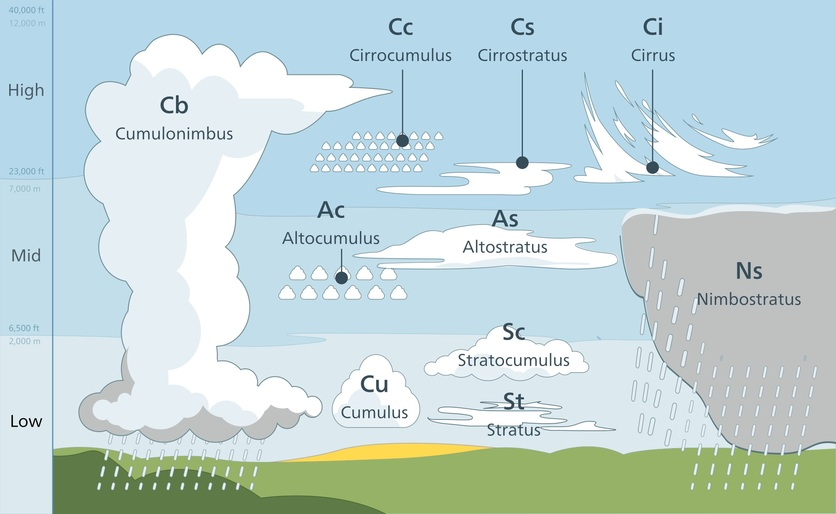
\includegraphics[width=\linewidth]{clouds-types.jpg}
    \captionof{figure}{Distinct classifications of cloudshapes in the troposphere \protect\cite{cloudtypes:wiki}.}
    \label{img:ui:mockup:live}
\end{figure}

\noindent
This graphic above provides and excellent overview of all distinct cloud types.
Each type is depicted in its signature shape and marked with the scientific name and abbreviation.
Natural clouds are typically identified by two major factors: shape and \gls{altitude}.
The \gls{altitude}, which is the distance from sea level to the cloud, is further split into three categories "low", "mid" and "high".
This corresponds to the altitude at which the cloud usually forms, up to twelve kilometers above ground. 
\\
All of those clouds are formed in the troposphere, Earth's lowest atmospheric layer.
Certain clouds may occur in the stratospheric or even the mesospheric layer, but they are usually a rare sight. Therefore, those clouds will not be covered in this project.

% refs:
% https://www.countryfile.com/how-to/outdoor-skills/how-to-predict-the-weather-forecast-using-clouds/
% NASA how do clouds form: https://climatekids.nasa.gov/cloud-formation/#:~:text=Clouds%20are%20created%20when%20water,are%20floating%20in%20the%20air.&text=That%20means%20some%20of%20the,drifted%20away%20into%20the%20atmosphere.
% NASA: https://www.nasa.gov/audience/forstudents/k-4/stories/nasa-knows/what-are-clouds-k4.html
% http://ww2010.atmos.uiuc.edu/(Gh)/wwhlpr/cold_front_precip.rxml?hret=/guides/mtr/cld/cldtyp/mdl/altcu.rxml
% https://content.meteoblue.com/en/meteoscool/weather/clouds/cloud-types

\pagebreak

\subsubsection{Cirrus}
\begin{wrapfigure}[10]{r}{6.3cm}
    \vspace{-\baselineskip}
    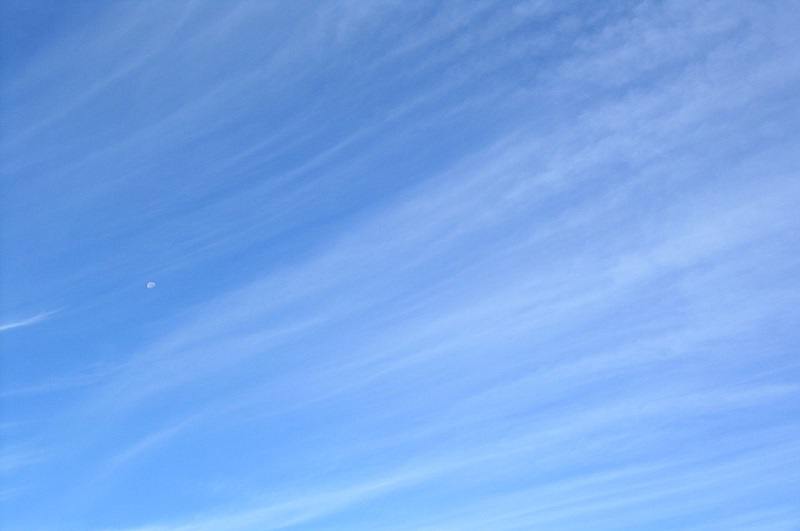
\includegraphics[width=6.3cm]{clouds/cirrus.jpg}
    \caption{Cirrus clouds \protect\cite{cloudtypes:wiki:cirrus}.}
    \label{img:clouds:cirrus}
\end{wrapfigure}
Cirrus clouds consist of thin, hair-like strands.
They fall into the "high" altitude group and mostly appear in a bright white color, although they may take on the colors of the sunset or sunrise.
Typically, they are formed when \gls{watervapor} undergoes \gls{desublimation}, the process in which gas turns into solid. This occurs when the \gls{watervapor} freezes rapidly at high altitudes, turning into ice crystals.
\\
\noindent
However, cirrus clouds can also form from air that flows outwards of thunderstorms.
\emptyline
\textbf{Interpretation:} Fair weather, but they might announce the arrival of \gls{warmfront} in 12-24 hours, which is often preceded by rain several hours in advance.
Even though cirrus clouds indicate \gls{precipitation}, they themselves do not produce rainfall \cite{predict:weather}.

\subsubsection{Cirrostratus}
\begin{wrapfigure}[10]{r}{6.3cm}
    \vspace{-\baselineskip}
    
\includegraphics[width=6.3cm]{clouds/cirrostratus.jpg}
    \caption{Cirrostratus clouds \protect\cite{cloudtypes:wiki:cirrostratus}.}
    \label{img:clouds:cirrostratus}
\end{wrapfigure}
Cirrostratus clouds are similar to the cirrus clouds, only that they are even thinner.
Those clouds depict more of a veil than a single cloud shape.
They form under the same conditions as the cirrus clouds and can cover a massive area of the sky, spanning thousands of kilometers.
\\
\noindent
Cirrostratus clouds sometimes produce white rings or arcs of lights around the sun or the moon called the \emph{\gls{halophenomenon}}.
Sometimes, the cirrostratus clouds are so thin that the halo is the only way to tell if there are cirrostratus clouds.
\emptyline
\textbf{Interpretation:} Fair weather, but they indicate a \gls{warmfront} within one or two days, bringing \gls{precipitation} \cite{cloudtypes:meteoblue}.

\subsubsection{Cirrocumulus}
\begin{wrapfigure}[10]{r}{6.3cm}
    \vspace{-\baselineskip}
    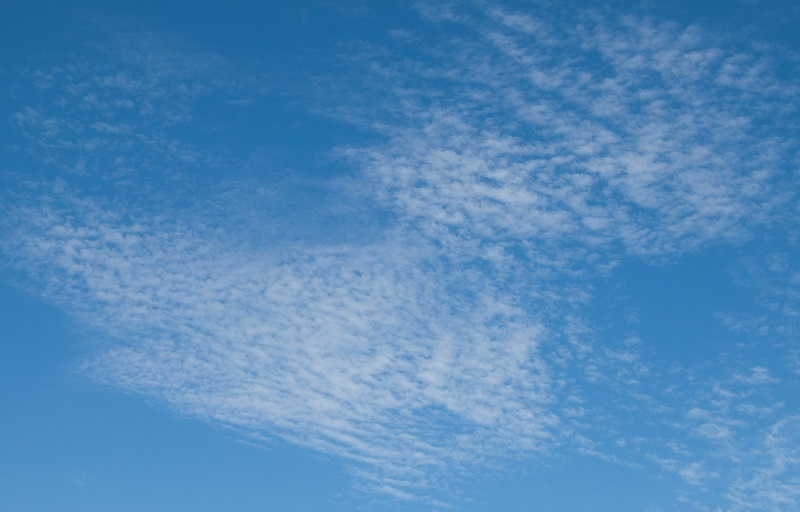
\includegraphics[width=6.3cm]{clouds/cirrocumulus.jpg}
    \caption{Cirrocumulus clouds \protect\cite{cloudtypes:wiki:cirrocumulus}.}
    \label{img:clouds:cirrocumulus}
\end{wrapfigure}
Similar to the other clouds of the cirrus-family, the cirrocumulus are composed of ice crystals and formed at high \gls{altitude}s.
They are made up of many small, white, puffy clouds called \emph{\gls{cloudlet}}s. Their wooly look give the cloud the name \emph{cumulus}.
\\
\noindent
Cirrocumulus clouds are realtively rare, as they are naturally only formed when a turbulent vertical current meets a cirrus cloud layer. The cirrus cloud then disperses into many \gls{cloudlet}s.
\emptyline
\textbf{Interpretation:} 
They do produce \gls{precipitation}, but it never reaches the surface, meaning that cirrocumulus clouds are typically associated with fair weather \cite{cloudtypes:meteoblue}.

\clearpage

\subsubsection{Altostratus}
\begin{wrapfigure}[11]{r}{6.3cm}
    \vspace{-\baselineskip}
    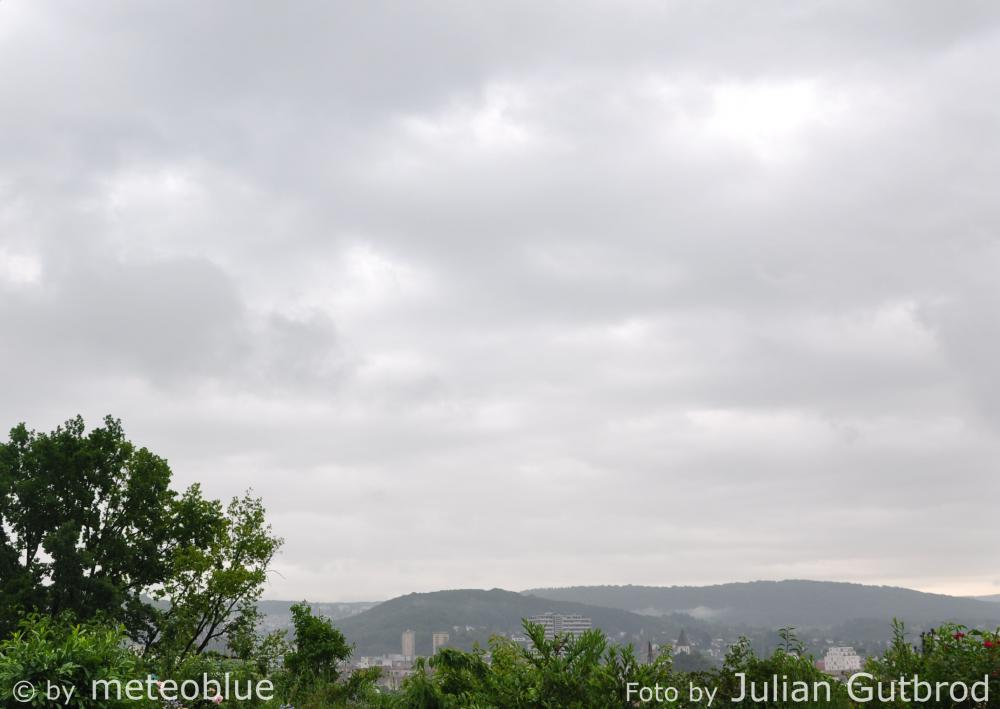
\includegraphics[width=6.3cm]{clouds/altostratus.jpg}
    \caption{Altostratus clouds \protect\cite{cloudtypes:meteoblue}.}
    \label{img:clouds:altostratus}
\end{wrapfigure}
The name for this grey, uniform sheet of clouds consists of the latin words \emph{alto} (height) and \emph{stratus} (layered), summing up their appearance accurately.
Altostratus clouds usually cover the whole sky and form a dull blanket of monocolored clouds with very few features.
The sun- or moonlight may shine through them, but will most likely not be strong enough to cast defined shadows.
\emptyline
\textbf{Interpretation:}
Altostratus clouds usually indicate \gls{precipitation}, even more so if they are are preceded by cirrus clouds.
If the \gls{precipitation} increases in persistence and intensity, the altostratus clouds will lower and thicken into nimbostratus clouds.


\subsubsection{Altocumulus}
\begin{wrapfigure}[9]{r}{6.3cm}
    \vspace{-\baselineskip}
    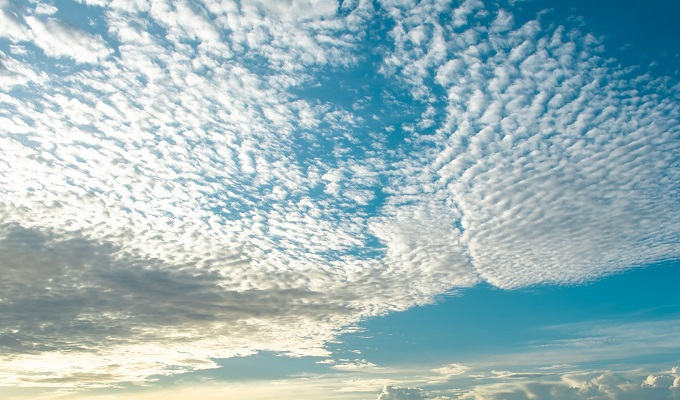
\includegraphics[width=6.3cm]{clouds/altocumulus.jpg}
    \caption{Altocumulus clouds \protect\cite{cloudtypes:wiki:altocumulus}.}
    \label{img:clouds:altocumulus}
\end{wrapfigure}
As with the cirrocumulus clouds, altocumulus clouds consist of small, puffy, white and grey \gls{cloudlet}s.
These \gls{cloudlet}s are usually slightly bigger than the ones of the cirrocumulus cloud.
It is easy to tell them apart, as the altocumulus \gls{cloudlet}s are usually more grey than white and are shaded on one side.
Altocumulus clouds can form through the dispersion of altostratus clouds or through \gls{convection} (see \sectionref{section:clouds:convection}).
\emptyline
\textbf{Interpretation:}
Usually, they are found in settled weather. They do not produce \gls{precipitation} that reaches the surface.


\subsubsection{Nimbostratus}
\begin{wrapfigure}[10]{r}{6.3cm}
    \vspace{-\baselineskip}
    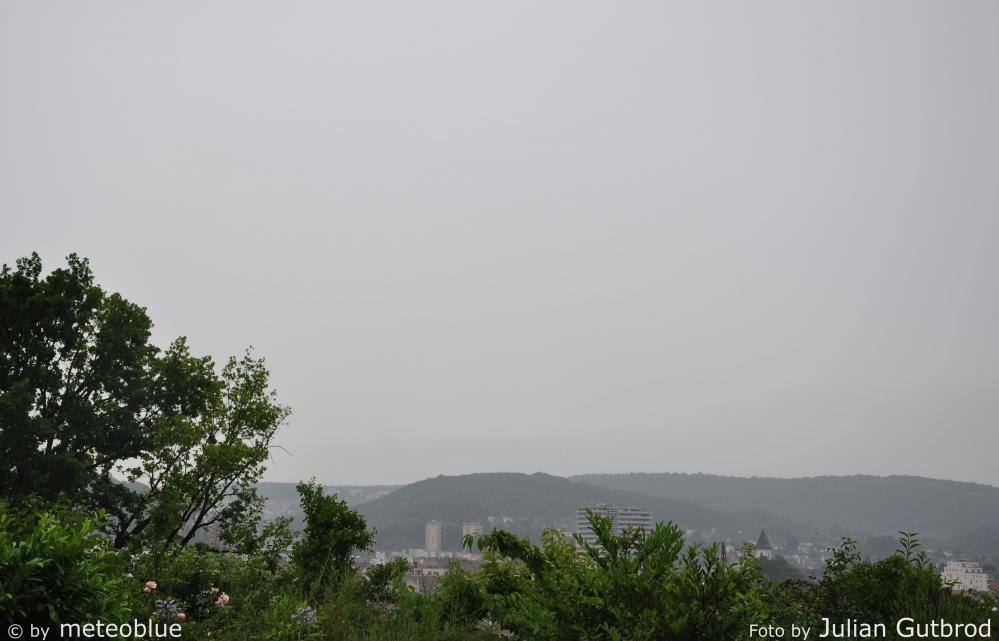
\includegraphics[width=6.3cm]{clouds/nimbostratus.jpg}
    \caption{Nimbostratus clouds \protect\cite{cloudtypes:meteoblue}.}
    \label{img:clouds:nimbostratus}
\end{wrapfigure}
The nimbostratus clouds are the vast, grey clouds that bring heavy rain or snow for a longer period of time, sometimes up to multiple days.
With their dark and gloomy appearance, they convey a dreary mood along with the persistent \gls{precipitation}.
\\
The thick, featureless layers of cloud are often formed by \gls{occludedfront}s, when an altostratus starts lowering and gets denser \cite{cloudtypes:wiki:nimbostratus}.
\emptyline
\textbf{Interpretation:}
They bring long-term rain or snow for several hours or days.

\pagebreak

\subsubsection{Stratus}
\begin{wrapfigure}[9]{r}{6.3cm}
    \vspace{-\baselineskip}
    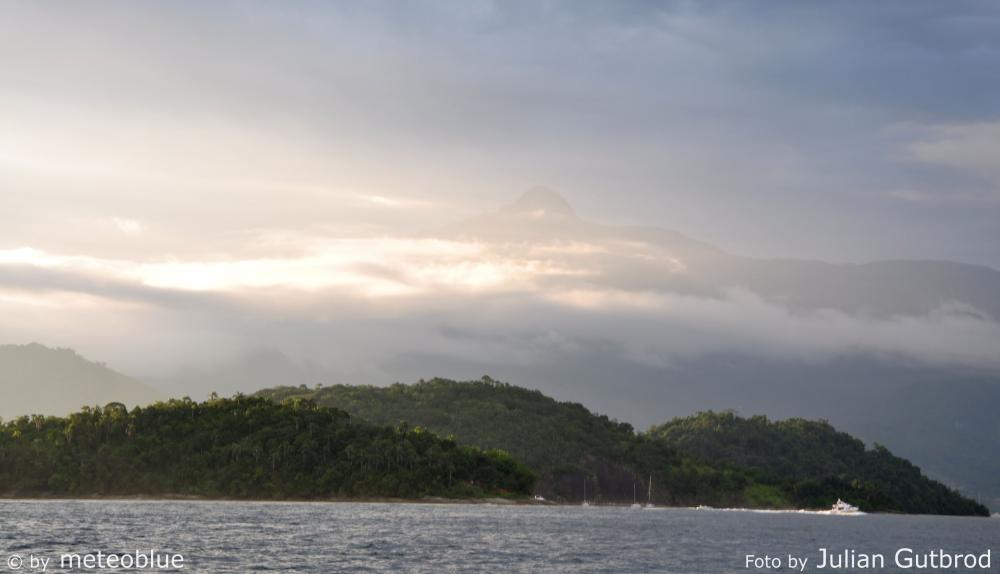
\includegraphics[width=6.3cm]{clouds/stratus.jpg}
    \caption{Stratus clouds \protect\cite{cloudtypes:meteoblue}.}
    \label{img:clouds:stratus}
\end{wrapfigure}
Stratus clouds are low-layer clouds that usually only form in calm, stable conditions.
They are often described as "high fog" as the have similiarities in appearance.
\\
Stratus cloud are formed by cool, moist air that is raised by mild wind breezes.
\emptyline
\textbf{Interpretation:}
They indicate quiet weather conditions, but sometimes produce sprinklings of rain.


\subsubsection{Cumulus}
\begin{wrapfigure}[10]{r}{6.3cm}
    \vspace{-\baselineskip}
    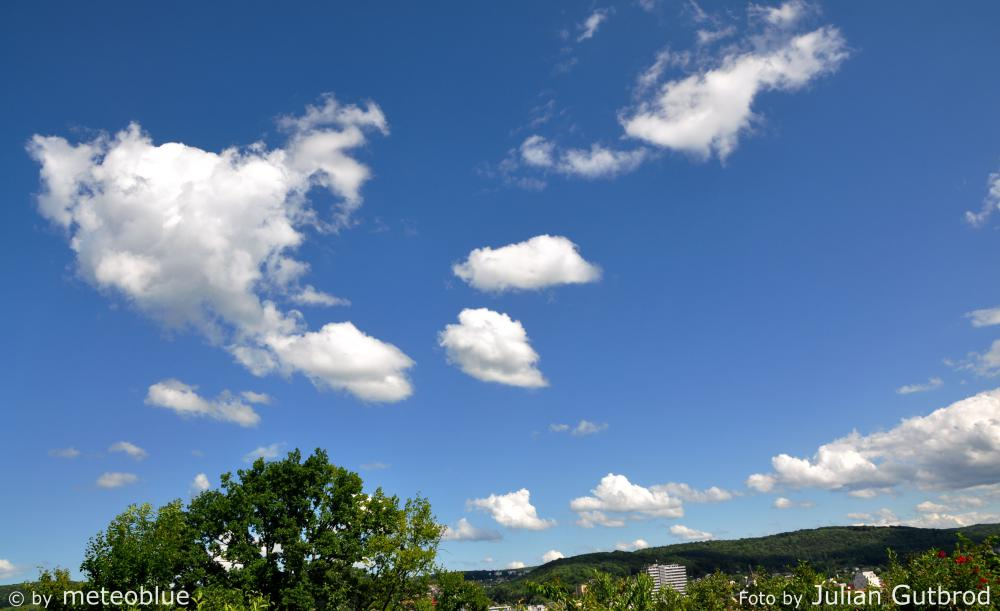
\includegraphics[width=6.3cm]{clouds/cumulus.jpg}
    \caption{Cumulus clouds \protect\cite{cloudtypes:meteoblue}.}
    \label{img:clouds:cumulus}
\end{wrapfigure}
Probably the most picturesque type of cloud is the cumulus. 
Its cotton-like look along with the soft, white color make it appear like candy in the sky.
\\
The individual heaps of cumulus clouds remain strictly separated.
The edge of each cloud is fuzzy and may change constantly.
\\
Cumulus clouds are almost exclusively formed by \gls{convection}.
This is why they are a good indicator for gliders and pilots that there are upward winds \protect\cite{cloudtypes:meteoblue}.
\emptyline
\textbf{Interpretation:}
They indicate fair weather, but can develop into cumulonimbus clouds, if weather conditions allow it.


\subsubsection{Stratocumulus}
\begin{wrapfigure}[10]{r}{6.3cm}
    \vspace{-\baselineskip}
    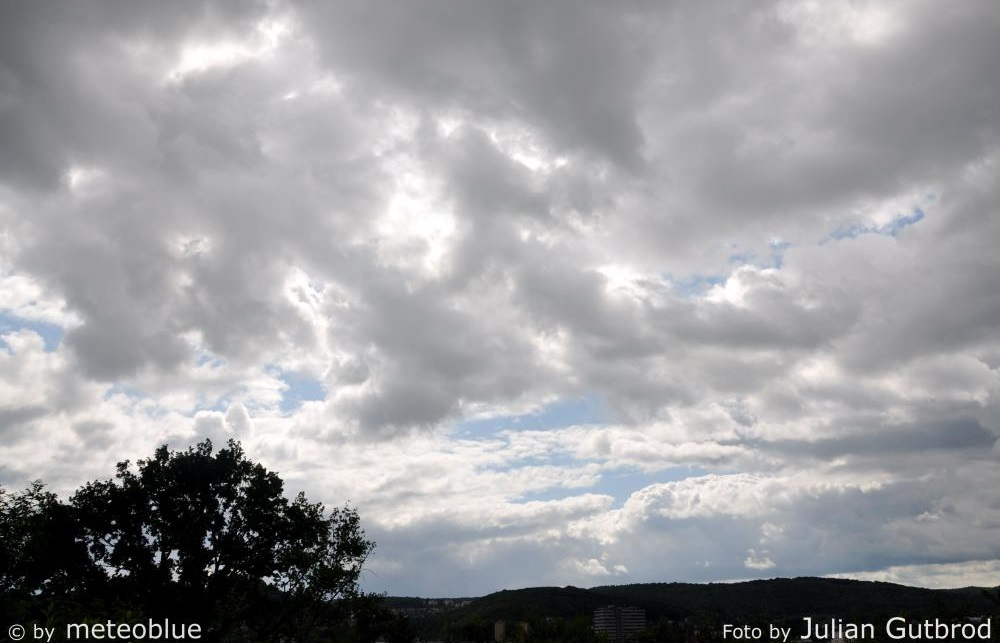
\includegraphics[width=6.3cm]{clouds/stratocumulus.jpg}
    \caption{Stratocumulus clouds \protect\cite{cloudtypes:meteoblue}.}
    \label{img:clouds:stratocumulus}
\end{wrapfigure}
These low-layer patches of cloud consist mainly of water droplets, absorbing a lot of light, giving them a saturated grey color.
\\
They are the most common clouds on Earth and usually form when there is a change in weather or when a layer of stratus cloud breaks up.
This means that stratocumulus clouds are present near cold, warm or \gls{occludedfront}s.
\\
Stratocumulus do not produce \gls{precipitation} themselves, but are formed in many different conditions, including rainy or calm weather.
\emptyline
\textbf{Interpretation:}
They announce an instability of the atmosphere and are usually present before an occlusion of weather fronts.

\pagebreak

\subsubsection{Cumulonimbus}
\begin{wrapfigure}[10]{r}{6.3cm}
    \vspace{-\baselineskip}
    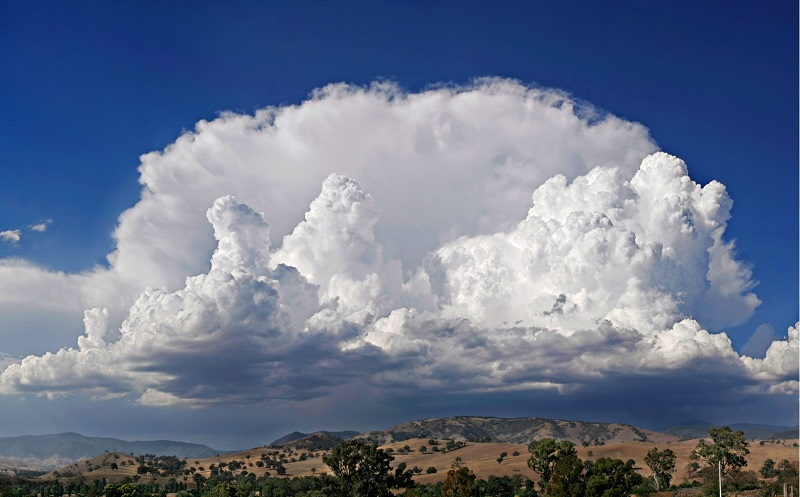
\includegraphics[width=6.3cm]{clouds/cumulonimbus.jpg}
    \caption{Cumulonimbus clouds \protect\cite{cloudtypes:wiki:cumulonimbus}.}
    \label{img:clouds:cumulonimbus}
\end{wrapfigure}
Cumulonimbus clouds are massive, high-towering heaps of cloud, spanning over the whole troposphere.
Their top is often shaped like an anvil, whereas the base if flat and dark, giving them a menacing look.
\\
They are referred to as thunderclouds, because they are the only type of cloud that is able to produce hail, thunder and lighting \cite{metoffice:cumulonimbus}.
\\
Cumulonimbus clouds are formed trough natural \gls{convection} or as a result of forced forced \gls{convection} when a \gls{coldfront} pushes up warm air.
\emptyline
\textbf{Interpretation:}
They cause extreme weather like heavy torrential rain, hail storms, lighting and even tornados.